% !TEX root = ./thesis.tex
\chapter{Integrating Stakeholders Perceptions of Connectivity Conservation Priorities into a Spatially Explicit Land Use and Connectivity Change Model}
\begin{center}
{Valentin Lucet$^{1}$, Andrew Gonzalez$^{1}$}\\
\end{center}
\textit{Author Affiliations:}\\
\normalsize{$^{1}$Department of Biology, McGill University}\\

\newrefsection

\section{Abstract}

Connectivity conservation science, whose goal is to preserve the continuity of habitat throughout a given landscape, proceeds by identifying priority areas given the current configuration of the landscape. However, current connectivity conservation planning methods often do not confront the results of the prioritization with the priorities perceived by stakeholders. There is a need for planning tools to allow for this confrontation to happen. The Montérégie region in southern Quebec, where this work takes place, is experiencing urban growth and sprawl, and stakeholders show an increasing interest in connectivity conservation tools. Those tools need to be able to guide stakeholders through an iterative process of conservation and land use scenario building. We take a first step toward deriving the basis for such community-driven scenarios and tools by presenting the results of a community workshop organized between multiple stakeholders in Montérégie. We use those results to derive simple land use change scenarios and use those scenarios to constrain the integrated model previously derived. We discuss the importance of considering stakeholder inputs to produce a resilient network of protected areas and highlight the need for a multi- stakeholder approach in the definition of conservation priorities. \\

\newpage

\section{Introduction}
%\textit{Problem statement}: Connectivity conservation planning methods do not account for stakeholder perceptions. This can potentially lead to ill-informed conservation plans with low chances of success.
%
%\textit{Research questions}: \textbf{How do different stakeholders perceive connectivity conservation priorities, given the obstacles and opportunities for land use planning apparent in the region, and which conservation scenarios can be derived from these perceptions?} \\

%-----------------------------------------------
% Intro paragraph, similar to that of from chapter 1

The goal of connectivity conservation planning is to preserve the continuity of habitat in a landscape, by identifying and protecting habitat patches and corridors necessary to maintain the movement of plants and animals \citep{keeley_thirty_2019}. Ecological connectivity, defined as the extent to which the landscape facilitates or impedes the movement of organisms \citep{crooks_landscape_2006}, is a critical component of the resilience of populations in heterogeneous and fragmented landscapes \citep{gonzalez_spatial_2017}. Connectivity conservation planning methods do not typically account for, nor confront the perceptions of stakeholders concerning connectivity conservation priorities. Here, we ask how those methods can progress by taking into account those perceptions. To do so, we integrate a connectivity and land use change model (developed in chapter 1) with the results of a community workshop organized with stakeholders, through simple conservation scenarios.

% CCP methods are increasingly Social-Ecological
Conservation planning methods are now recognizing that landscapes constitute social-ecological-systems. A social-ecological system (SES) can be understood as the ensemble of human and non-human actors in a given landscape, the set of natural habitats they inhabit and resources they use, and the set of interactions that are maintained between all the components of the system \citep{ostrom_general_2009}. SESs thus form complex and integrated aggregates of interactions \citep{hinkel_enhancing_2014}. Those interactions also impact governance, the process by which actors in power establish rules and laws \citep{bissonnette_comparing_2018}. To understand a landscape as an SES has important implications for land use planning and therefore for connectivity conservation planning, and pushes connectivity scientists to integrate stakeholder’s perceptions and priorities into their models. 

% Why is it important to integrate perceptions
It is important to integrate the perceptions of stakeholders in connectivity planning methods for a multiplicity of reasons. It engages stakeholders in the planning process early on, contributing to better consensus on priorities and, hopefully, to faster action. It also means that connectivity models are enriched by integrating local knowledge into the decision making process, showing that inputs from stakeholders are valued and considered essential to build a conservation plan. More specifically, connectivity conservation is often faced with the issue of understanding the processes driving land use change \citep{worboys_connectivity_2010}. Because land use change is a social process with consequences of both social and ecological nature, questions of land use and connectivity planning cannot be answered without input from stakeholders. Recent studies in land use modeling have shown the value of using stakeholder’s inputs for parameterizing and validating models \citep{hewitt_participatory_2014, voinov_modelling_2010}, leading to a much better understanding of land use processes at play within a landscape.

Connectivity conservation research therefore has a lot to gain from the wide set of participatory research methods already being used in social-ecological research. Participatory research methods are designed to conduct the research process “with those people whose life-world and meaningful actions are under study” \citep{bergold_participatory_2012}. Participatory research methods can include scenario design. A scenario is “an account of a plausible future” \citep{peterson_scenario_2003}, and scenario design is a flexible tool for conservation scientists and practitioners. Although scenarios are often derived from expert knowledge, they can be built in a participatory setting. In this context, it is often conceived by researchers as an iterative process, through which scenarios are imagined, reviewed and re-imagined in a set of stakeholder meetings with the goal to build consensus on the desirability of each scenario. 

Scenarios have been widely applied in conservation research, both at global \citep{tscharntke_global_2012, brussaard_reconciling_2010}, regional and local \citep{carlson_scenario_2011, delevaux_scenario_2018} scales. In a participatory setting, other methods can be used to help in scenario design: those methods include participatory mapping, a participatory GIS method. Participatory mapping involves leveraging the knowledge that stakeholders hold about the geography of their landscape, in order to achieve a community-driven objective. It has been widely used in social-ecological research \citep{plieninger_assessing_2013, lynam_review_2007}. 

% Why PM can be beneficial 
Participatory GIS methods such as participatory mapping can allow connectivity conservation models to be more spatially explicit about the obstacles and opportunities presented by connectivity conservation. Understanding how these obstacles and opportunities can influence management decisions is crucial for our understanding of connectivity conservation planning, where land-use conflicts can hinder the protection and restoration of connectivity. Although it is relatively easy to identify where land-use changes might conflict with connectivity conservation, evaluating to which extent these conflicts matter in a local conservation context is more difficult \cite{mitchell_monteregie_2015}.

Here we do not present a scenario design exercise, but a community workshop with a consensus building and participatory mapping exercise, whose results were engineered as simple scenarios in an integrated land use, climate change, and connectivity model (developed in chapter 1). We improve our understanding of the obstacles and opportunities to connectivity conservation in the region, and provide a good starting ground for an iterative process of scenario building. We focused on the region of Montérégie, in southern Quebec, where connectivity conservation has become the focus of land use planning decisions. This project has been developed in collaboration with the non-profit NAQ (Nature action Quebec) in the context of a multi-stakeholder conservation project, the PADF (Plan d’Aménagement Durable des Forêts). The PADF aims at building consensus on priorities for the management and possible conservation of forested land in the region.

% We build on mitchell
This research is pursued in continuation of the project “Monteregie Connection”, whose goal was to engage stakeholders around a discussion of the ecosystem services provided by natural habitat in the region. In the context of this stakeholder-driven project, \cite{mitchell_monteregie_2015} conducted a non-spatially explicit scenario building exercise for a subset of the Monteregie region, the Vallée-de-Richelieu Municipalité Region Comté. The outcome was the 4 scenarios, going from “Periurban Development” to “Green Development”, describing different land use change trends. The Monteregie connection project improved our understanding of the relationship between forest connectivity and ecosystem services. However, there was no effort to estimate the impact of each scenario onto the ecosystem services. This is partially due to a lack of tools able to translate these scenarios into simulations. We contribute to the development of such tools by integrating the results of the workshop into the land use change model developed in chapter 1. The goal of this chapter is therefore twofold: gain a better understanding of conservation priorities in the region, and to provide a basis for an iterative scenario-building process. 
\\
%-----------------------------------------------

\section{Methods}

In order to understand what stakeholders perceive as a conservation priority, and derive conservation scenarios from those perceptions, we conducted a community workshop. The workshop was approved by McGill University’s Research Ethics Board (see appendix {x} for the approval letter). The workshop was held on January 22nd 2020 in the public library of Saint-Jean sur Richelieu. \\

\subsection{Community workshop}

The workshop aimed to gather stakeholders from multiple groups:
\begin{enumerate}
  \item Representatives of Non-Governmental Organizations that are involved in the conservation of ecological connectivity within the study extent (i.e. Montérégie).
  \item Land use planners (“amenagistes”) of the administrative regions covered by the study extent (the 15 MRCs in Montérégie).
  \item Representatives of Ministries involved in conservation (MFFP, MELCC).
  \item Representatives of the UPA (“Union des producteurs agricoles”) in Montérégie.
  \item Representatives of the private forestry industry unions (“producteurs forestiers”)
\end{enumerate}
Of all the groups, only the last group was not represented. \\

\subsubsection{Consensual mapping}

We employed a method coined “consensual participatory mapping in geographically structured focus groups”. Participants whose organisations operate in the same region (the same MRC) were seated at the same table. See table \ref{tab:workshoptables} for the breakdown of each MRC by table. In addition, for participants whose zone of influence or zone of action covered the whole region, two “regional tables” were created. In the subsequent sections, the workshop results are divided between the regional and regional tables.
The general method proceeded in 3 exercises, each step involving the same focus groups.

\begin{itemize}
  \item Exercise 1: mapping of forested cores of importance for ecological connectivity.
  \item Exercise 2: mapping of obstacles (for example: specific land use types, development projects in progress, local legislation) and opportunities for habitat connectivity in terms of social-economic activity and land use.
  \item Exercise 3: mapping of links (already recognized or potential) of importance between forested cores of importance, taking into account obstacles and opportunities on the landscape.
\end{itemize}

Each of these three exercises was conducted in 4 to 5 steps. Here we use exercise 1 to describe the method in more detail at each step.

\begin{enumerate}
\item Individual reflection - each participant thought on their own about the problem at hand. For instance, participants took time to think about what forested cores are important to connect in the landscape
\item Group discussion, at each table (i.e. in each focus group) each participant contributed their answer to the question posed by the exercise. For instance, participants shared what forested cores they found to be important.
\item Group discussion on the criteria that each participant used to answer the question. For instance, participants said why they thought they chose these forested cores.
\item Consensus building, participants voted for the most important criteria. For instance, participants used stickers that identify their group affiliation to vote for the criteria they found most important.
\item Room discussion: all participants exchanged on their decisions by sharing the results of their table’s work to the rest of the room.
\end{enumerate}

Each participant received a unique and neutral identifier of the form Affiliation-Geography. For example, a (hypothetical) land use planner from the table that brought together participants from the Maskoutains region received the code [A-1-1], and the UPA representatives from the Richelieu region received the codes [C-3 -1] and [C-3-2]. In addition, for certain activities, the affiliation of the participants is color-coded. For instance, blue for the land use planners and purple for the ministry representatives.

The coding system manifests itself in multiple ways, depending on the activity:
\begin{itemize}
\item When participants engage in activities involving drawing, the materials on which they draw will bear the aforementioned coding (A-1 etc..).
\item When participants engaged in activities involving post-its, the color of their post-it represented their affiliation or bore the aforementioned coding, depending on the activity.
\item When participants engaged in activities involving a weighting of choices with stickers, the color of their post-it or sticker represented their affiliation or had the aforementioned coding, depending on the activity.
\end{itemize}

To ensure that this system is used consistently throughout the workshop, each participant was given a personal folder with their own color-coded stickers and post-its. Participants were instructed to only use the stickers and material that have been personally handed to them. All participants were given a visual aid to remind them of the agenda of the workshop. Facilitators were also present at almost every table and helped facilitate the discussion. They were given a document to help them in this role. All workshop materials, including the ethics approval document for this research project can be found in Appendix 2.\\

\subsubsection*{Weighting system}

 The participants were given a total of 6 stickers to cast their vote for the opportunities and obstacles that they thought were most important. They were given a total of 6 stickers: 2 blue (important), 2 yellow (very important) and 2 red (of the first importance).\\

\subsubsection{Data processing and analysis}

\subsubsection*{Voting: opportunity and challenges}

The data from the opportunities and challenges activity (with post-its), and the weighting of these elements were treated with the following steps:
\begin{enumerate}
  \item Each post-it (opportunity or challenge) received a unique ID.
  \item A first score is calculated by summing the points for each sticker (each vote)
  \begin{itemize}
      \item 1 point for a blue vote
      \item 2 points for a yellow vote
      \item 3 points for a red vote
  \end{itemize}
  \item This score was then weighted by multiplying it by the post-it’s diversity score which served as a measure of consensus
\begin{itemize}
\item This diversity score is the inverse simpson index (R package Vegan). The more diverse the group the higher this index is.
\end{itemize}
\end{enumerate}
These steps were carried out for each table and the results were treated separately for each table because not all tables had the same potential for diversity. For each table, the 10 post-its with the highest scores were retained, 5 among the post-its that had been placed on a specific area of the map (spatialized) and 5 for those that were not. The list of post-it contents, along with the scores, can be found in the appendix tables \ref{tab:opp_chall_ns} and \ref{tab:opp_chall_s}. In addition, a map synthetic map of the spatialized post-its was produced (see figures \ref{fig:reg_AC} and \ref{fig:trans_AC}).\\

\subsubsection*{Digitization of results}

The priority areas and links were digitized by hand in QGIS. The smooth tool was used to generalize the trace of each area and corridors (see figures \ref{fig:reg}  and \ref{fig:trans} for the final results). It is important to note that those maps are an approximate representation of reality, as the drawings done during the activity were an approximation of what the participant had in mind.

In order to integrate the results with the land use change model, we added a 5 km buffer around the linkages to simulate a corridor effect. This corridor width size is arbitrary and is in most cases  an unrealistic expectation forhow large a wildlife corridor can or should be. \\

\subsection{Conservation and land use change scenarios}

The conservation scenarios were derived with the goal to demonstrate how results of this type of community workshop can be integrated with other planning methods for connectivity conservation, such as land use change and connectivity modelling. They are not meant to be directly used as conservation guidelines. They are unrealistic by definition and are meant to reflect the most extreme bounds of connectivity change and/or protection measures imaginable for the region. More realistic scenarios featuring targeted action would need to be devised in future community workshops. Although there exists a tremendous amount of work on scenario-building for conservation, specific examples for connectivity conservation are rare. The scenarios presented here are a “proof of concept” for the integration of qualitative results into a quantitative model. 

We integrated the results of the workshop with the land use change and connectivity model devised in Chapter 1 by changing two attributes of the model: \textit{conservation status} and \textit{reforestation location}. These additional conservation scenarios are crossed with the climate change scenarios.

Conservation status determines whether or not forest can be cut down, and whether pixels can transition into urban and agricultural land. In Chapter 1, we gave this status to areas that were previously known as protected, but assumed no more forest would be added to this set of protected areas. In this chapter, a protection status is given to all pixels within the identified priority areas and within a 5km buffer around the identified priority linkage areas. All pixels under this status cannot transition into urban land and remain in their state. This represents an unrealistic proportion of the region under protection (about 33% of the region)

The reforestation status modified what zones can be targeted for reforestation. In reforestation scenarios in Chapter 1, reforestation happened randomly (barring some neighboring rules). In this chapter, reforestation is targeted to the same areas identified in the workshop (all pixels within the identified priority areas and within a 5km buffer around the identified priority linkage areas). As in the model described in Chapter 1, all new reforested area takes the value of medium aged (30-50 yr) deciduous forest and remain in this state for the rest of the simulation. As previously mentioned, this assumption is necessary because LANDIS surface types are not available for newly forested areas. For the same reason, no forest transitions are allowed for this forest type. These two assumptions are conservative:  we do not impose succession or disturbance on these newly forested ares and assume medium age as an average age class.

The three modified conservation and land use change scenarios are therefore:
\begin{enumerate}
  \item Business as usual land use change + corridor protection \textbf{(BAU-Corr)}
 \item Business as usual land use change + corridor protection + reforestation \textbf{(BAU-R-Corr)}
 \item Business as usual land use change + corridor protection + targeted reforestation \textbf{(BAU-R(T)-Corr)} \\
\end{enumerate}

\subsubsection{Connectivity analyses}

In order to be able to compare the results of these new scenarios with those developed in Chapter 1, we conducted the same connectivity analyses using the Circuitscape software. The software “borrows algorithms from electronic circuit theory to predict connectivity in heterogeneous landscapes''. It is a free and open software under MIT license developed originally in Python, and now in its 5th version, in Julia \citep{circuitjulia}.

For each of the maps produced in the suitability analysis, Circuitscape was run in two directions (“wall to wall” run, \cite{mcrae_conserving_2016}): east to west and north to south. This method allowed us to model omnidirectional animal movements, and required that we added the resulting North/South and East/West flow map. The results for each map were therefore added to produce a final set of flow maps for analysis. From these flow maps, we extracted the mean flow for each of the municipalities and for the entire flow map. 

In addition, similarly to in Chapter 1 we extracted the distribution (logged) of pixel flow values under the form of histograms. We also ran the SURF analysis in the same way and counted up the number detected feature for each surface, in order to derive a measure of flow complexity.\\

\section{Results}

\subsection{Community workshop}

During our community workshop, participants identified connectivity conservation priorities in Monteregie. Participants quickly built consensus on which key cores areas and corridors should be prioritized for protection or restoration. They mainly identified large forested regions and protected areas as key cores areas. As key corridors, participants were strongly drawn to linear strips of connecting “stepping-stone” patches. They were rarely drawn to redundant corridor design. When participants were asked what factors would make a link a priority, they emphasized the quality of habitats to be linked, as well as a diversity of constraining and facilitating factors.

Participants also workshopped constraints and assets to connectivity conservation in Monteregie. We divided the results into elements that had been spatialized (i.e. placed on a specific location of the map during the exercise), and non spatialized (i.e. not placed on a specific location ), and scored them for the level of consensus they generated. Constraints scored higher, on average, than assets, indicating a focus of participants on constraints. The elements in the spatialized set scored higher on average than in the non spatialized set, indicating that participants tended to focus on more tangible and local issues and assets.

Non-spatialized elements seemed to speak to more general and large scale aspects. The main theme among these elements was predominance of agriculture in the landscape, and the difficulties to reconcile agricultural production with conservation. On the other hand, spatialized elements seemed to reflect local realities for connectivity conservation, such as the presence of highways or specific trends in land use change such as villegiative pressures. \\

\subsubsection{Forested cores of importance} 

Protected areas are well represented in the identified key core areas, for example the protected areas of the Green Mountains in the MRC of Brome-Missisquoi, or parts of the Monteregian Hills such as the Mount Saint-Hilaire. 

The participants at the sub-regional (figure \ref{fig:reg_AC}) and regional (figure \ref{fig:trans_AC}) tables identified redundant groups of forest patches. Because regional tables covered the whole of Monteregie, they often identified cores that contained the cores identified by the sub-regional table. \\

\subsubsection{Obstacles and assets}

The tables identified a total of 63 items as opportunities or assets, and 56 as constraints or obstacles. Tables \ref{tab:opp_chall_s} and \ref{tab:opp_chall_ns} displays the 5 assets or obstacles that scored the highest for each workshop table. 

Non-spatialized elements seemed to speak to more general and large scale aspects. Among them, the assets that scored the highest varied according to the sub-region under consideration. In the Centre table participants emphasized the strong presence of environmental NGOs, whereas the North and East tables emphasized elements linked to forest management. Interestingly, the presence of a strong agricultural matrix in the region scored high as an asset at the regional tables, and very high as a constraint on a sub-regional table, highlighting the polarizing status of the agricultural land use type in the region. Another constraint linked to agriculture is the CPTAQ - an agency responsible for the protection of agricultural lands often involved in discussions around land use planning - mentioned for the Centre sub-region. Similarly, the East table mentioned the issues that farmers have to make their farm profitable as another constraint. Besides agriculture, participants emphasized other constraints, such as economic realities making conservation a less likely investment, given the cost of implementing connectivity conservation measures - also mentioned as a perceived constraint. Finally, the participants mentioned that the overwhelming majority of forests are situated on private lands, along with the existing road infrastructure.

Spatialized elements seemed to reflect local realities for connectivity conservation. They are summarized in maps \ref{fig:trans_AC} and \ref{fig:reg_AC}, which shows the single highest scoring element (asset or constraints) for each sub region. the Centre, East and North tables mentioned positive local inclinations toward conservation. Similarly, the West and regional tables mentioned local legislation and the active mobilization of stakeholders, highlighting that connectivity conservation is a concern for many stakeholders in the region. Concerning constraints, participants emphasized once again elements related to the predominance of agriculture in the region. The lack of engagement from farmers was mentioned in the Centre and West tables, along with land use "pressures" coming both from agriculture and urban spread. The East table emphasized on the similar "villegiative" pressures, along with more local concern such as the Highway 10 and the intensity of local agriculture practices. The North table also mentions its highways. The regional tables mentioned the price of agricultural lands and the need for compensating the loss of agricultural production due to conservation. \\

\subsubsection{Links of importance at the regional scale}

\subsubsection*{Factors of priority}

Among the factors that were designated as a priority for the identification of links, participants emphasized the characteristics of the natural environments that make up the nodes that are to be connected. They mentioned the importance of the "quality" of these nodes themselve: for instance, the protection status of habitats, their diversity (variety of habitats), their surface area, isolation or proximity, and the pre-existence of connectivity potential. This highlights that stakeholders agree on the value of high quality habitats and on the need to protect them.

Participants debated the importance of both "facilitating" and "constraining" factors in deciding whether a link is a priority. Facilitating factors included the feasibility of establishing the link, social facilitators such as political and social buy-in, and territorial facilitators, such as appropriate land use. There were several types of constraints: financial, social, territorial and physical, and must be considered in relation to the socio-political and spatial planning context in which they emerge. % example?

The presence of species at risk was identified as an important factor, along with other elements such as social factors (available economic means and the level of local interest in conservation) and characteristics of the link itself, including the functionality of the corridor. Consideration of threats such as the level of fragmentation was also noted. Finally, the fact that the environment is to be protected or restored was also deemed important. Interestingly, regulations are among the factors that were cited less often, such as Quebec's PRMHH ("Plans régionaux des milieux humides et hydriques", or regional wetlands conservation plans), and migration routes. \\

\subsubsection*{Priority link mapping}

The consensual mapping process identified important links between the key areas identified in the previous steps at both sub-regional (figure \ref{fig:reg}) and regional tables (figure \ref{fig:trans}). At sub-regional tables, participants displayed what could be called "corridor opportunism": participants wanted to link areas by joining patches they judged to be organized in a linear or corridor-like fashion.

Participants were rarely drawn to redundant corridors. Tables were asked to limit themselves in the amount of links they were to prioritize, but were not given an exact number. Only one table (North) felt that corridor redundancy was important enough to include redundant design in their priorities. It can be clearly seen in figure \ref{fig:reg} most participants decided to sacrifice redundancy for parsimony, as only the northern part of the region displays redundant (yet arguably still parsimonious), corridor design.

As for the forested cores, there was a lot of redundancy between links identified at the sub-regional and regional tables. Because the regional tables covered the entire region, they were able to identify links at a larger scale (see figure \ref{fig:trans}). This allowed the participants to designate a larger scale link along the Saint Lawrence River, as well as links between the lake Champlain region and the easternmost parts of the region, and between the Saint-Francois wildlife area and mount Rigaud, mentioning that this last link would need to be implemented in collaboration with Ontario. It was clear that participants at regional tables felt that a broader discussion of links with outside of the region was necessary. \\

\subsection{Conservation scenarios}

\subsubsection{Land use change model}

The projected land use maps for each of the conservation scenarios allowed us to visualize some of the possible futures for the region, if connectivity conservation, as it is conceived by the participating stakeholders, were to become a priority for regional land use planning. Figures \ref{fig:Corr_compare}, \ref{fig: CorrRef_compare} and \ref{fig: CorrRefT_compare} compares land use maps from 2010 with the projected maps for 2100 for each of the conservation scenarios.

The information contained in those maps is summarized with a bar chart showing changes in Agricultural, Urban and Forested land use area for 2010 and 2100 (see figure \ref{fig:bar_chap2}). For all scenarios, the urban area was allowed to almost double. This is apparent in all maps, where urban land has spread in a similar fashion to the BAU scenario in Chapter 1. Forest is maintained for all scenarios except for the BAU-Corr scenario, which only differs from the BAU scenario of chapter 1 in that the links and areas identified by stakeholders are protected from urbanization and agricultural expansion. In this scenario, agriculture is also allowed to maintain its area. This is not the case for the other scenarios, which include reforestation, which, in the context of spreading urban land, must result in the loss in agricultural land (similarly to what was observed under the reforestation scenario in Chapter 1).

Although the two conservation scenarios that include reforestation do not differ in their changes to the different land use area, they display different spatial patterns. Under the BAU-R-Corr scenario we observe a similar pattern of growing forest patches than under Chapter 1's Reforestation scenario : small patches have disappeared (except in the corridors) and bigger patches have grown. But we see the most striking difference with the last conservation scenario, BAU-R(T)-Corr, for which reforestation is targeted to the corridors identified by the stakeholders. Under this scenario, we still assume that forests grow from existing patches. The consequence of these two constraints is that where forest can grow easily in a linear fashion, it tends to do so. Therefore we see that corridors of forest are delineated, within the 5km buffer around identified links that were given to the model. The pattern is especially striking in the north of the region. In the south and the west of the region, we see a different pattern under which the model generated the growth of the identified forested cores. \\

\subsubsection{Connectivity modelling}

\vspace{1em}

\subparagraph*{\textit{Current flow}} The three conservation scenarios impacted the mean flow values for our five species differently, but we can derive a few common patterns from figures \ref{fig:flow_linear_2} (linear graph) and {\ref{fig:flow_radar_2} (radar graph). In comparison to the species BAU scenario (for which the responses are described in Chapter 1), we see that the conservation scenarios usually manage to slow the decrease in mean flow. As in chapter 1, only the black bear (\textit{Ursus americanus}) - and, to some extent, the short-tailed shrew (\textit{Blarina brevicauda}) - manage to maintain a similar level of mean flow under the conservation scenarios that include reforestation.

In terms of decrease in mean flow, the smallest departure from the outcome predicted by the BAU scenario is observed in the BAU-Corr scenario (protection of identified areas). The mean flow at the end of the simulation is systematically better than for the BAU, but always worse than the two other conservation scenarios, except under RCP 8.5 climate for the american marten, for which the outcome is on par with the BAU scenario under baseline climate.  Similarly to chapter 1, we see that some species's response is more linear than others, but in general all species under all scenarios (except for the BAU scenario) show some curving in their response. it is important to note that the conservation of areas and links of importance is only triggered in 2020  - not at the start of the simulation in 2010 - which could contribute to the non-linearity by providing a point of inflection in the response.

We can note the variations on which of the two reforestation scenarios is most effective at curbing the decrease in mean flow, the degree of which tends to depend on the climate scenario as well as the species. For the wood frog, random reforestation performs better than targeted reforestation, invariant on climate. Same pattern for the redbacked salamander, but for it warming scenarios are consistently better and lead to less loss in mean flow. For the back bear, the two reforestation scenarios ended with the same amount of loss in 2100 (despite some early divergence), and did not depend on the climate scenario. The flow values for the short-tailed shrew also decrease less under the random reforestation scenario, and displays larger differences between historic and climate change scenarios. Finally, the most complex patterns are observed for the american marten.  Although it also seems to do better under random reforestation,  the response varies with the climate scenario; the response curves are staggered in such a way that targeted reforestation under the baseline climate scenario predicted higher mean flow than random reforestation under RCP 8.5. Similarly, the BAU scenario under baseline climate predicts higher flow values than the BAU-Corr scenario under RCP 8.5. This highlights an apparent non-linear response to climate by the american marten, for which baseline climate seems worse than RCP 8.5 but better than historical change.

\vspace{1em}

\subparagraph*{\textit{Flow distributions}} In chapter 1, we showed the importance of looking beyond the mean flow values and searching for patterns in how the distribution of flow values change. We also characterized two different effects on those distributions: a "directional" effect, which acted to shift high flow pixels toward lower flow intensities, and a "polarizing" effect, which pushed middle level values toward low values, with small to no effect on high value pixels.

In the conservation scenarios of this chapter we see that the BAU-Corr scenario has a clear directional effect across all species' histograms (see figure \ref{fig:hist_2}) toward smaller flow values, whereas the other two scenarios which include reforestation have a polarizing effect, similarly to in Chapter 1. However, in the case of the black bear, we see a directional shift toward more positive values.

\vspace{1em}

\subparagraph*{\textit{Feature detection}} The results of the feature detection via SURF vary a lot depending on the species. The simplest response is from the black bear, for which, as in Chapter 1, less features are lost in scenarios without reforestation (there was no apparent impact of climate) than in scenarios with reforestation. The redbacked salamander and the wood frog responses were similar: less features are lost in scenarios without reforestation, but differences between scenario outcomes are more strongly marked and we see an effect of climate, with warming scenarios leading to more losses in features. The responses of the short-tailed shrew and the american marten are more complex. Although for the shrew, scenarios without reforestation seem to lead to the loss of fewer features, the curves are bundled in such a way that differences are less stark. Finally, the american marten shows the opposite pattern: scenarios without reforestation lead to more losses in features than scenarios with reforestation. In addition, there is a hierarchical pattern between the outcomes of the different climate scenarios: warming scenarios lead to more losses in features than the historic scenario (absence of climate change).\\

\section{Discussion}

Conducting participatory research in Monteregie led us to a better understanding of the obstacles and assets to connectivity conservation in the region. The predominance of the agricultural land cover and its implications for land use planning and the regional economy was revealed as the most important source of obstacles for the region’s conservation goals, but also as a source of opportunities to develop more biodiversity-friendly farming practices. The expansion of urban infrastructure ranked high in more forested regions of the landscape. A range of assets was identified in the region: the strong engagement of local actors in connectivity conservation was a key factor. Through a consensual mapping workshop, we also mapped consensual priority core areas and links, showing how participants think corridors should make the best use of linear strips of the remaining forest in the region. Specifically, this demonstrates that participants saw small patches as important for corridor design and perceived corridors as an important tool to conserve and restore the potential of fragmented patches. However, it also means that designing corridors in such a way might mean that an otherwise important patch could be ignored because its location does not fit a linear corridor design. 

Interestingly, Different tables also identified corridors with variable redundancy. Redundancy is an important connectivity conservation design, increasingly being explored in connectivity experiments \citep{fletcher_matrix_2014}. It is possible that participants at the north table though redundancy was necessary to make the best use of the layout of forest, which are interspersed in the agricultural matrix. This is by opposition to the corridors of the south table, where forest patches are smaller and more scarce. Participants at this table might have thought that one non redundant linear corridor was all they could ask for in a predominant agricultural matrix. Those results represent a first step toward a better model of how stakeholders could make complex conservation-related decisions. 

The integration of those corridors to the land use change model shows how qualitative priorities from a participatory process can be turned into model inputs. It is interesting to see that some changes anticipated by workshop participants are observed in our land use change business as usual scenario. For instance, the increasing land development in the east of the region toward estrie, coined as “villegiature pressure” by participants to designate the building of cottages and country houses. This demonstrates that participants are in tune with current land use change in the region and that our model was able to replicate them. Concerning connectivity results, it is important to see how they compare to the business as usual scenario. These results complement those of chapter 1 and show similar patterns with regards to species response. When only looking at mean flow values, species with linear and simple response are those who seem to depend on forest types that are only under threat by land use change. On the other hand, species dependent on forest types that are under threat both by land use change and climate change show a more complex response, with more variations in the final outcome (2100 horizon) of the scenarios. 

Concerning flow complexity, it is interesting to note that the number of features detected by the SURF algorithm is consistently lower through time for all species under targeted reforestation (in corridors) - except for the Marten. It is possible that corridors allow to streamline current flow and prevents complexification that arises with fragmentation, although, as pointed out in chapter 1, the link between number of features and and complexity would need to be examined in more details before drawing a final conclusion. 

We extend on the work of \cite{albert_applying_2017}, which implemented a simple land use change model, but did not attempt to generate any alternative scenarios. In many ways, this work can be compared to recent work that looked at how connectivity could change under a range of scenarios. One example is \cite{rubio_sustaining_2012} who tested whether a network of forested patches resilient to different land use change scenarios, for a species of nuthatch. They found that although identifying such a network was possible, its effectiveness and efficiency was under threat under certain scenarios. Our results suggest that findings of that sort are likely to change when climate change is considered, if the species under study is dependent on sensitive forest types. 

The results of our simple scenarios have implications for connectivity conservation in the region. The reforestation scenario suggests that reforesting as much land as is urbanized is what is necessary to maintain mean current flow. But this is only one simple measure of connectivity, and therefore those results suggest that more work is needed to explore which metric would be most appropriate to look at in this context, and more importantly what land use practices (protection, reforestation, urban densification) would be enough to maintain this metric. In the light of the results from our workshop, it is clear that reforesting the same amount that we are urbanizing is possibly socially unacceptable, given the amount of agricultural loss it generates. Even such a simple scenario echoes the long debated question of land sparing versus land sharing, a dichotomy that is now largely questioned as it fails to address the complexity of both food systems and the diversity of farming practices \cite{tscharntke_global_2012, bennett_changing_2017}. In fact our reforestation scenario can be seen as an agricultural intensification model, in which farmers are able to cultivate less land to allow for more space for forest. Yet our workshop results suggest that stakeholders would not think along those lines, and are more likely to propose compensations to farmers for the loss in productive surface or for changes in practices. This is likely reinforced by the fact that some stakeholders are opposed to further intensification of agricultural practices (also cited as an obstacle by participants). New compensation schemes such as ALUS (Alternative Land Use Services) are being experimented in Monteregie and are looking promising in their capacity to federare a bottom up movement of conservation in agrosystems \cite{ouellet_community_2020}. 

The simple approach to the sparing vs sharing question that is brought about by our scenario overlooks the question of scale. At the scale of Monteregie, it is unclear to which extent the reduction in agricultural land can be promoted by the regional government. Like all modern farming systems, Quebec's agriculture is embedded in a global market which might make it likely to prioritize global trends over local interests. Therefore, we are overlooking important variables for the design of credible alternative scenarios for conservation in the region, variables that are more likely to be elucidated in a participatory setting like the one we used.

Our methodology would allow us to explore alternative scenarios with ease. We imagined simple scenarios and therefore served as an intermediary between the workshop output and the model inputs. However, given the flexibility of the STSIM land use change model framework, steps could be taken to reduce that distance between stakeholders outputs and model inputs. The interest of stakeholders in participating in our workshop demonstrates that local actors are longing for tools that allow them to close the loop between what they think should be done and what it would effectively mean for species on the ground, to explore where and how much reforestation would provide the optimal corridor design, or how much redundancy is really needed. To make this a reality, we are missing some knowledge about specific parameters - for instance, what the ideal width of a corridor for a given species, or how much agricultural loss is acceptable to reforestation. But we are also missing specific tools, and this project demonstrates that it is now easier to get there. The STSIM framework has been used in a participatory setting before. For instance, in \cite{jarnevich_developing_2019}, STSIM was used to produce a model for invasive species spread and fire management, using expert knowledge collected in a participatory setting. The authors also highlight the value to be found in involving “end users” of model results (i.e. stakeholders) in the modelling process. There remains a lot of work to be done to put these analyses in the hands of stakeholders. Making the analysis open and the code reproducible is one step in this direction.

Perhaps the most important limitation of this work is the fact that the strong consensus which was quickly built during the workshop is fragilized by the absence of some key stakeholders which, in spite of being invited, were not able to partake in the activity. This further illustrates the need for consensual mapping and the need for an iterative process with the goal to involve a larger diversity of stakeholders. Participatory research scholars have discussed the importance to consult and involve a diverse set of participants, representative of different knowledge systems, in efforts of participatory modelling \cite{gray_modeling_2012}. The lack of representatives from the forestry and farming industries, important stakeholders in forest management, limits the impact of consensus building. 

Similar limitations to those raised in chapter 1 also apply. For instance, the habitat suitability analysis, and the analysis of flow surfaces have important flaws that would need to be addressed (see chapter 1 for more details). Another critique could be made about the targeted reforestation scenario: due to the parameterization of the reforestation, it was easier for patches in the north of the region to grow into linear strips of corridors. This happened at a lower rate in the southern part of the region, due to the lack of the pre-existing patches of forest. Future scenarios will need to test if allowing for new patches to spawn on the map produces the same outputs - as long as this land use change trend is thought likely by stakeholders. 

\section{Conclusion}

Through participatory research we demonstrated the value of stakeholder engagement to models of connectivity conservation planning. We contributed a better understanding of obstacles to connectivity conservation and highlighted the flexibility of a scenario approach for the consideration of alternative scenarios of land use planning and connectivity conservation. Under our community-based scenarios, we observed similar types of response (linear versus nonlinear, simple versus complex) in our study species. Although we provided a basis for an iterative framework of community-driven scenario building, future research will need to achieve better representation in stakeholder groups. 

%---------------------------------------------------------------------------------------------------------------------------------------------------

\newpage
\begin{center}
\section*{Figures \& Tables}
\end{center}

%---------------------------------------------------------------------------------------------------------------------------------------------------
% tables (moved to appendix)

%---------------------------------------------------------------------------------------------------------------------------------------------------
% figures

% AC

\begin{figure}[h!]
\makebox[\textwidth]{
\includegraphics[width=1.3\textwidth]{thesis/figures/Regional_AC.png}
}
\caption{Cartography of opportunity and challenges  with the highest importance and diversity metric (for sub-regional tables) - summary from workshop results.}
\label{fig:reg_AC}
\end{figure}
\clearpage

\begin{figure}[h!]
\makebox[\textwidth]{
\includegraphics[width=1.3\textwidth]{thesis/figures/Transversal_AC.png}
}
\caption{Cartography of opportunity and challenges  with the highest importance and diversity metric (for regional tables) - summary from workshop results.}
\label{fig:trans_AC}
\end{figure}
\clearpage

%------------------------------- - --------------------------------------------------------------------------------------------------------------------
% Links and areas

\begin{figure}[h!]
\makebox[\textwidth]{
\includegraphics[width=1.3\textwidth]{thesis/figures/Regional.png}
}
\caption{Cartography of priority areas and links (for sub-regional tables) - summary from workshop results.}
\label{fig:reg}
\end{figure}
\clearpage

\begin{figure}[h!]
\makebox[\textwidth]{
\includegraphics[width=1.3\textwidth]{thesis/figures/Transversal.png}
}
\caption{Cartography of priority areas and links (for regional tables) - summary from workshop results.}
\label{fig:trans}
\end{figure}
\clearpage

%---------------------------------------------------------------------------------------------------------------------------------------------------
% Land use composition

\begin{figure}[h!]
\makebox[\textwidth]{
\includegraphics[width=1.3\textwidth]{thesis/figures/bar_chap2.png}
}
\caption{Land use class frequencies in 2010 (observed) and 2100 (predicted) for the BAU and conservation scenarios (under baseline climate scenario).}
\label{fig:bar_chap2}
\end{figure}

%---------------------------------------------------------------------------------------------------------------------------------------------------
% Flow radar all moved to appendix

% Linear
\begin{figure}[h!]
\makebox[\textwidth]{
  \includegraphics[width=1.3\textwidth]{thesis/figures/connectivity_decrease_x5species_chap2.png}
}
 \caption{Change in mean flow (in \% of the the 2010 flow) between 2010 (observed) and 2100 (predicted), contrasting BAU scenario (solid line) with other conservation scenarios - linear graph.}
 \label{fig:flow_linear_2}
\end{figure}

% Radar
\begin{figure}[h!]
\makebox[\textwidth]{
  \includegraphics[width=1.3\textwidth]{thesis/figures/radar_ggradar_chap2.png}
}
 \caption{Change in mean flow (in \% of the the 2010 flow) between 2010 (observed) and 2100 (predicted), contrasting BAU scenario (solid line) with other conservation scenarios - radar graph.}
 \label{fig:flow_radar_2}
\end{figure}

% Histograms
\begin{figure}[h!]
\makebox[\textwidth]{
  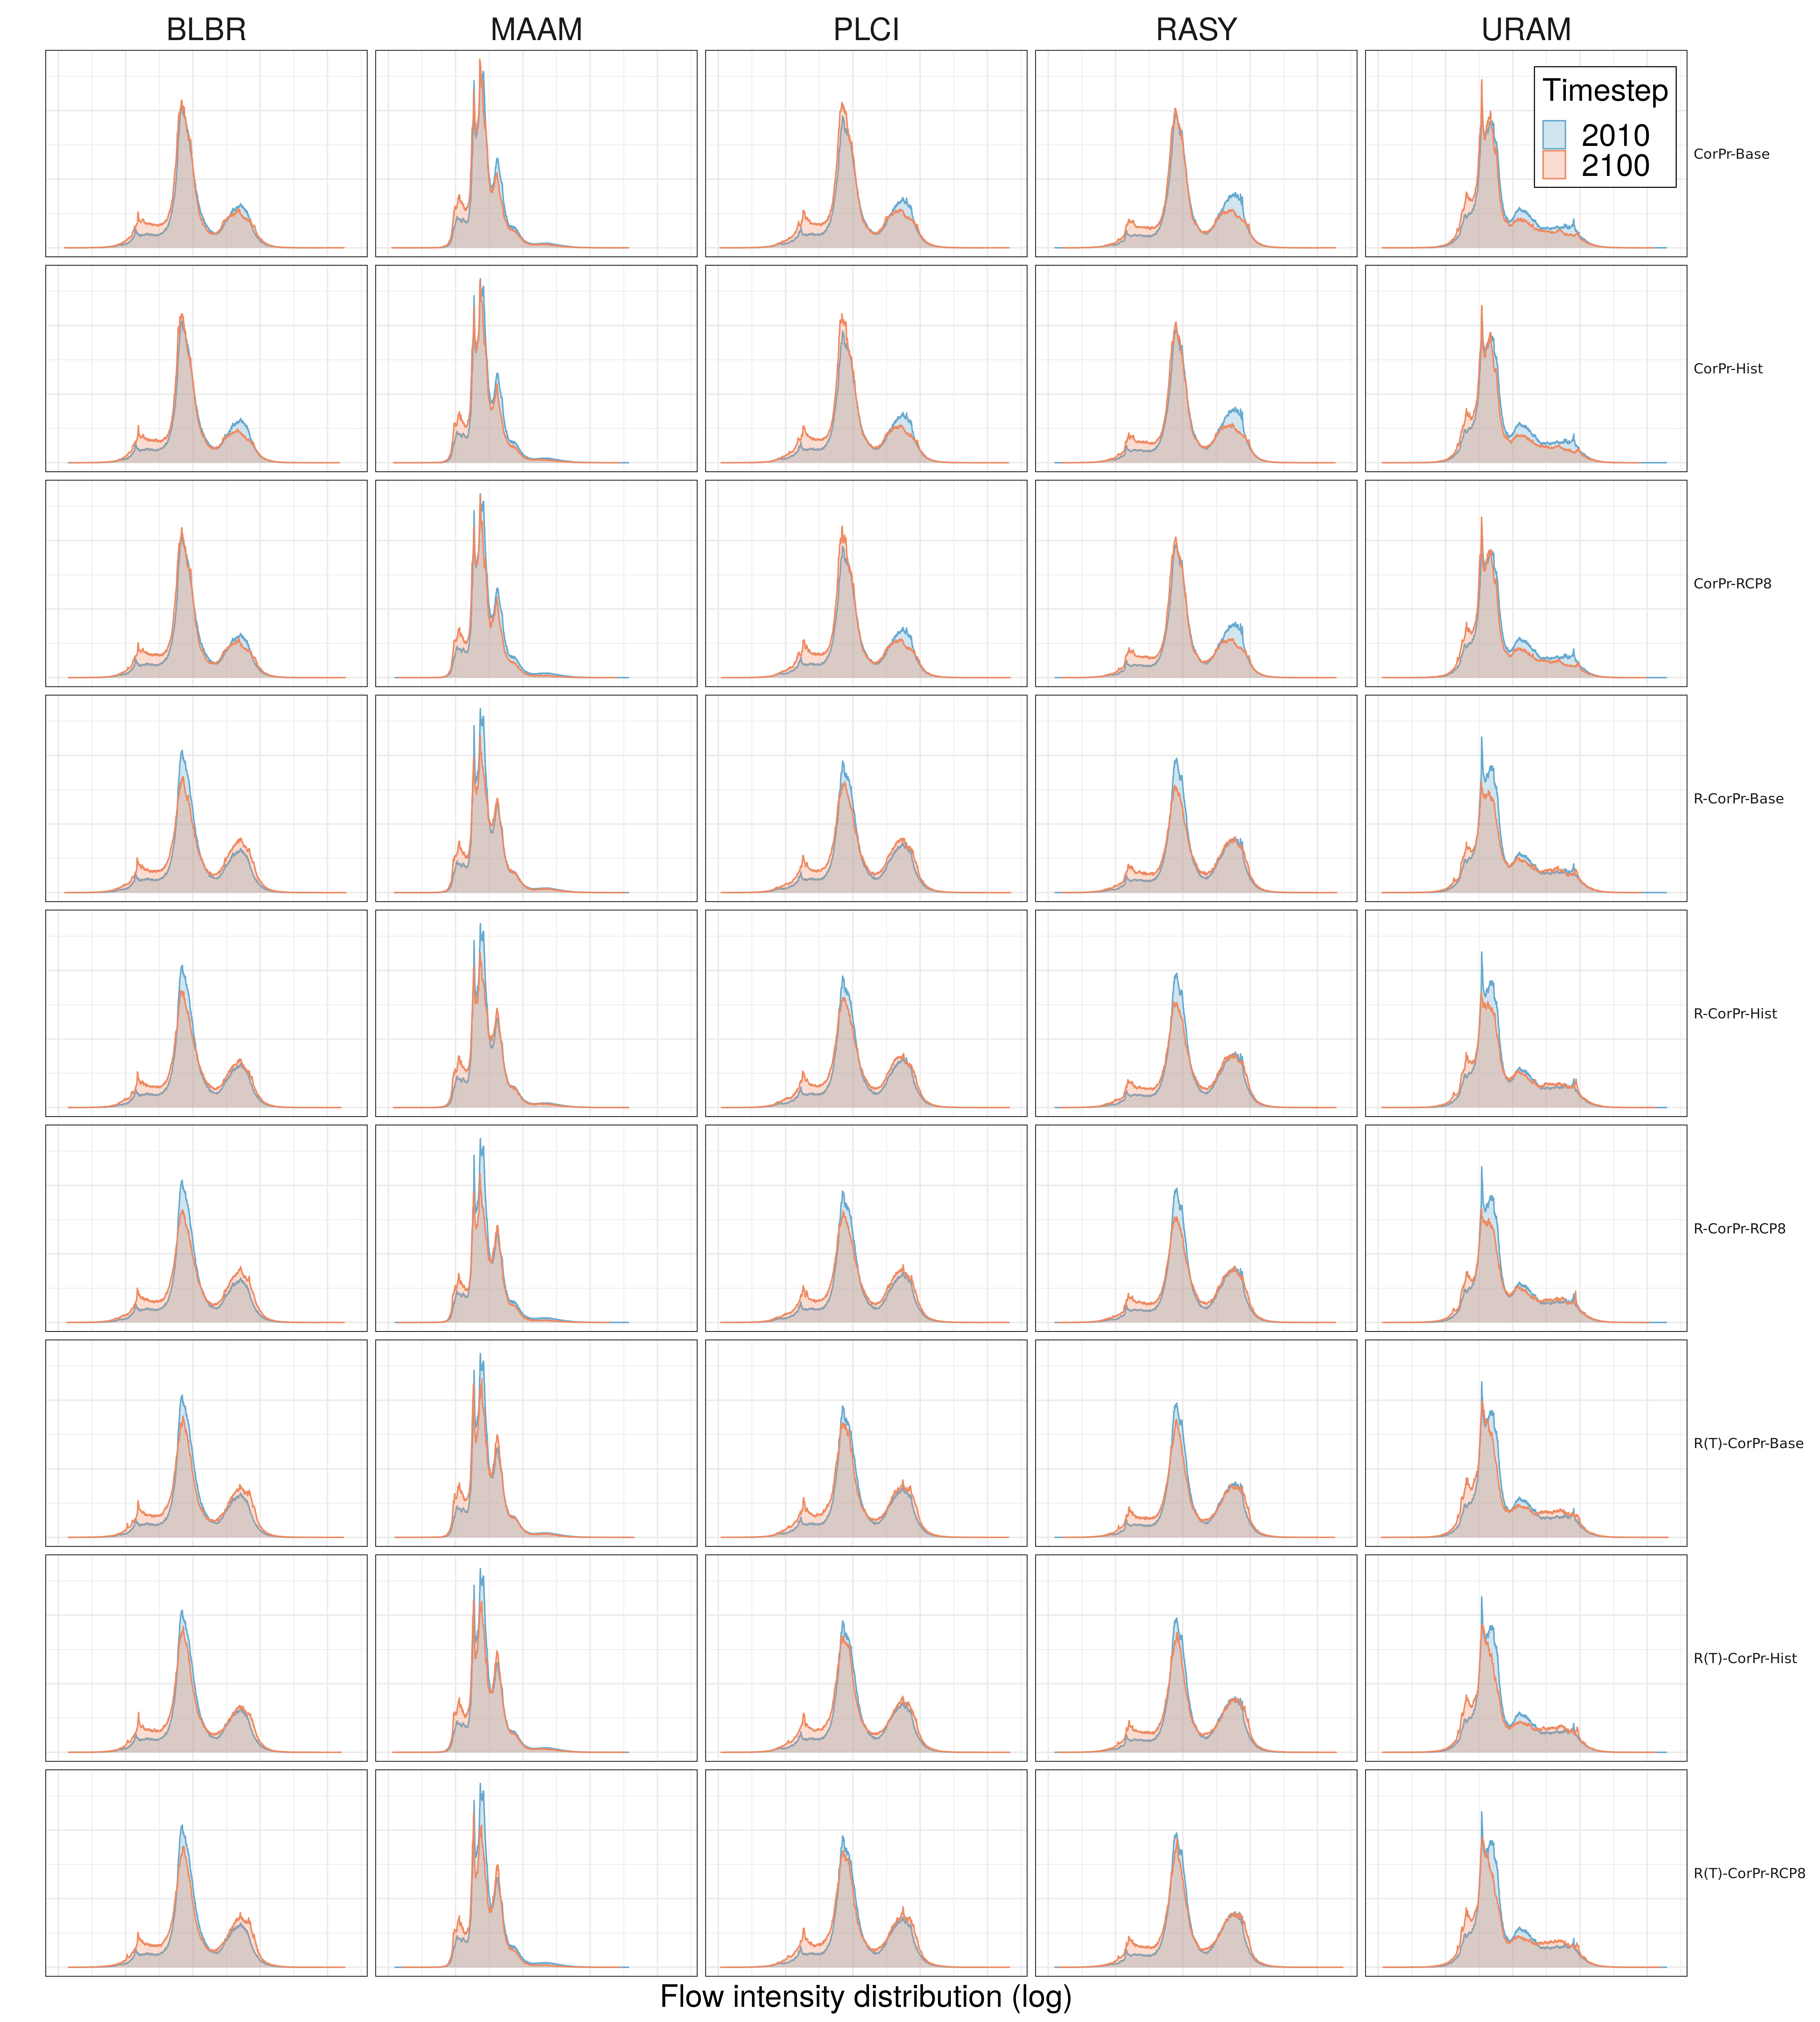
\includegraphics[width=1.3\textwidth]{thesis/figures/hist_chap2.png}
}
 \caption{Histograms of flow values for all species and scenarios, for 2010 (observed) and 2100 (predicted).}
 \label{fig:hist_2}
\end{figure}

%---------------------------------------------------------------------------------------------------------------------------------------------------
% SURF

% Linear
\begin{figure}[h!]
\makebox[\textwidth]{
  \includegraphics[width=1.3\textwidth]{thesis/figures/surf_chap2.png}
}
 \caption{Change in the number of features (in \% of the the 2010 flow) identified by the SURF analyssis between 2010 (observed) and 2100 (predicted), contrasting BAU scenario with other conservation scenarios - linear graph.}
 \label{fig:surf_linear_2}
\end{figure}

% Radar
\begin{figure}[h!]
\makebox[\textwidth]{
  \includegraphics[width=1.3\textwidth]{thesis/figures/surf_radar_chap2.png}
}
 \caption{Change in the number of features (in \% of the the 2010 flow) identified by the SURF analyssis between 2010 (observed) and 2100 (predicted), contrasting BAU scenario with other conservation scenarios - radar graph.}
 \label{fig:surf_radar_2}
\end{figure}

\printbibliography[heading=bibintoc, section=2, title={Chapter 2 Bibliography \hspace{1em}}]

\endrefsection

\newpage